% Previous work into shearing bijels have demonstrated how particles prefer to move in the direction of shear and if strong enough, even detach from the interface. \cite{bonaccorso_shear_2020} It has also been shown how at curved interfaces, ellipsoidal particles  

\section{Introduction}

While the microstructure and synthesis techniques for bijels have been explored in earnest, the rheology of bijels
has remained relatively unexplored. Some interesting phenomena for bijels and shearing include the 
presence of monogels, made by remixing the phase separated liquid domains of the bijel while the electrostatic
interactions between particles maintains the structure of the particle monolayer. \cite{sanz_colloidal_2009} 
Monogel formation has been observed in lutidine/water and styrene/butadiene oligomer based bijels but not ethane-diol nitromethane based bijels
\cite{sanz_colloidal_2009, bai_dynamics_2015, tavacoli_novel_2011} Computational Investigations have identified that confined bijels under shear undergo elongation of
the domains in the direction of shear succeeded by particle detachment from the interface and eventual failure of the bijel. \cite{bonaccorso_shear_2020}
More recently, bijels have been identified to be 2D glasses percolating in 3D space, characterized through comparing the complex rheology of bijels against
colloidal gels made from silica particles with electrostatic interactions. \cite{ching_bijel_2022} 

In many of the manufacturing techniques outlined the rheological properties are essential in ensuring that 
the casting mixture remains processable. \cite{haase_continuous_2015,haase_situ_2016} In STrIPS, the flow rate of the casting mixture and the co-solvent
control the microstructure of the bijel and the morphology of the resulting bijel material, controlling whether droplets or ropes are synthesized. \cite{haase_continuous_2015}
When investigating the effect of magnetic fields on the rheological properties of suspensions, it has been shown that the viscosity of ferrofluids increases substantially due
to the self assembly of particles restricting the flow of fluid, greatly increasing the viscosity of the ferrofluid. cite{qiao_magnetorheological_2012} The application
of shear onto suspensions can also cause shear banding as interparticle interactions mediate particle fluid interactions, creating localized velocity differences to the bulk.
\cite{xu_relation_2013} Looking into emulsions, the application of magnetic fields increases the viscosity of emulsions, making them more shear thinning than when no field 
is applied.

In past chapters, I identified the microstructure and particle arrangement of bijels stabilized by ellipsoidal particles under magnetic fields and demonstrated
particles morphology specific ordering to the applied magnetic field. I also show that the local ordering of the particles is affected from the application of
the magnetic field. In this chapter, I probe the dynamics of bijels under constant shear to understand how these microstructural and particle monolayer changes
affect the rheology of bijels stabilized by ellipsoidal particles under magnetic fields. First, I define a shear capillary number 
$Ca_s = \frac{\eta_{f} \dot{\gamma} R_s}{\sigma}$ where $\dot{\gamma} = \frac{2u_{LE}}{L_x}$ is the
strain rate and $R_s$ is the size of equivalent spherical particle. \cite{frijters_effects_2012, yang_capillary_2022} In the literature, $Ca_s$ has been between between 0.04 
and 0.16. However, the box size in these simulations were smaller, meaning that these capillary number ranges would exceed the 
maximum mach number the model allows if this same range were used $(Ma \leq 0.03)$. To accommodate this limitation the 
largest capillary number used will be $Ca_s = 10^-4$ which correspond to a maximum of $Ma \approx 0.02$. As all particles used 
have only hard-sphere type interactions, it is expected that the behaviour seen should mimic 2D colloidal glasses 
percolating in 3D space, akin to what Ching and Mohraz saw, with an additional dependence on the direction of shear. 
This would predict the discovery of particle monolayer dependent elasticity and yield stress along with shear thinning 
behavior of the bijels.

To verify these predictions, bijel microstructure will be defined using four processing histories; The first is of a 
bijel simulated under a $\Bar{B} = 1$ magnetic field strength, the second is a bijel stimulated under no field, 
followed by the application of a $\Bar{B} = 1$ field after jamming, the third is a bijel simulated under no field, 
while the final microstructure is a bijel simulated under $\Bar{B} = 1$ magnetic field, followed by switching the 
field off after jamming. This gives insight into the impact of processing history on the shear properties of a bijel, 
in addition to the microstructural and colloidal insights gained. Based on the results in Bonaccorso et al., there 
should be shear driven and shear rate dependent elongation of the domains in the direction parallel to the applied 
shear which in this system will be seen as a reduction in $L_{\perp}$ and an increase in $L_{\parallel}$. 
\cite{bonaccorso_shear_2020} The microstructure anisotropy will also be a factor in the viscosity results, as 
larger domains are more permeable than smaller ones, meaning that bijels where $L_{\perp} > L_{\parallel}$ should 
see less of the domain elongation effects shown in Bonaccorso et al. as the permeability of the bijels rises with 
larger domain size. \cite{bonaccorso_shear_2020}

It is also expected that the effective viscosity will be different between the four microstructures dependent upon the 
degree of nematic ordering and microstructural anisotropy of the bijel. Nematic ordering of the particles in the direction of shear
should resulting in a lowered effective viscosity compared to bijels without nematically 
ordered particles. \cite{xu_relation_2013, vermant_flow-induced_2005} Tracking of the proportion of particles on the 
interface will also yield insight into how the packing of the particles affects the rate at which particles will get 
ejected from the interface. Bonnacorso et al. identified that shear applied onto bijels caused particles to align to the direction of
shear before being ejected from the interface. Systems with a larger $\eta_{eff}$ are predicted to have the largest domains, largest 
difference between initial and final particle order and lowest number of particles left on the interface once steady 
state has been established. 

\section{Results}\label{sec:results_p3}

I begin this investigation by analyzing the rheological response of bijels stabilized by ellipsoidal particles under constant shear.
Specifically, I investigate the effect that particle order has on the rheological response characterized. I am also interested in
identifying the impact that the application of magnetic fields have on the rheological response of the bijel. 
Bijel templates simulated in Aim 1 with no field and a field strength of $\bar{B} = 1$ stabilized with a prolate and oblate particles with a 
particle volume fraction $\phi_p = 0.15$ were used as the starting point for these simulations. Next, I apply a field strength of
$\bar{B} = 1$ or switch off the applied field to all structures. This results in four processing setups; $\bar{B}:0\rightarrow 0$, $\bar{B}:0\rightarrow 1$,
$\bar{B}:1\rightarrow 0$ and $\bar{B}:1\rightarrow 1$. I then define a shear capillary number,  $Ca_s = \frac{\dot{\gamma} R_{s} \eta_{f}}{\sigma}$ where 
$\dot{\gamma}$ is the applied strain rate, $R_s$ is the equivalent spherical radius of the particles, $R_s = 7.9$, $\eta_f$ is the dynamic viscosity of the 
fluid and $\sigma$ is the surface tension of the interface. I use five shear numbers, $Ca_s = 1\cdot10^{-4}, 5\cdot10^{-5}, 1\cdot10^{-5}, 5\cdot10^{-6}, 1\cdot10^{-6}$.

\subsection{Viscosity measurement}

The ordering of the particles play an important role in determining the rheology of suspensions as ordered particles can slip over one another
before the structure breaks. The adsorption of particles on the interface of a bijel could affect how this slip occurs. Previous work investigating
the rheology of bijels have determined shear thinning behavior characterized with a Herschel-Buckley fit equation. \cite{macmillan_rheological_2019} 
I perform this analysis on the structures I have simulated. First, I plot the shear stress over time.

\begin{figure} 
    \centering 
    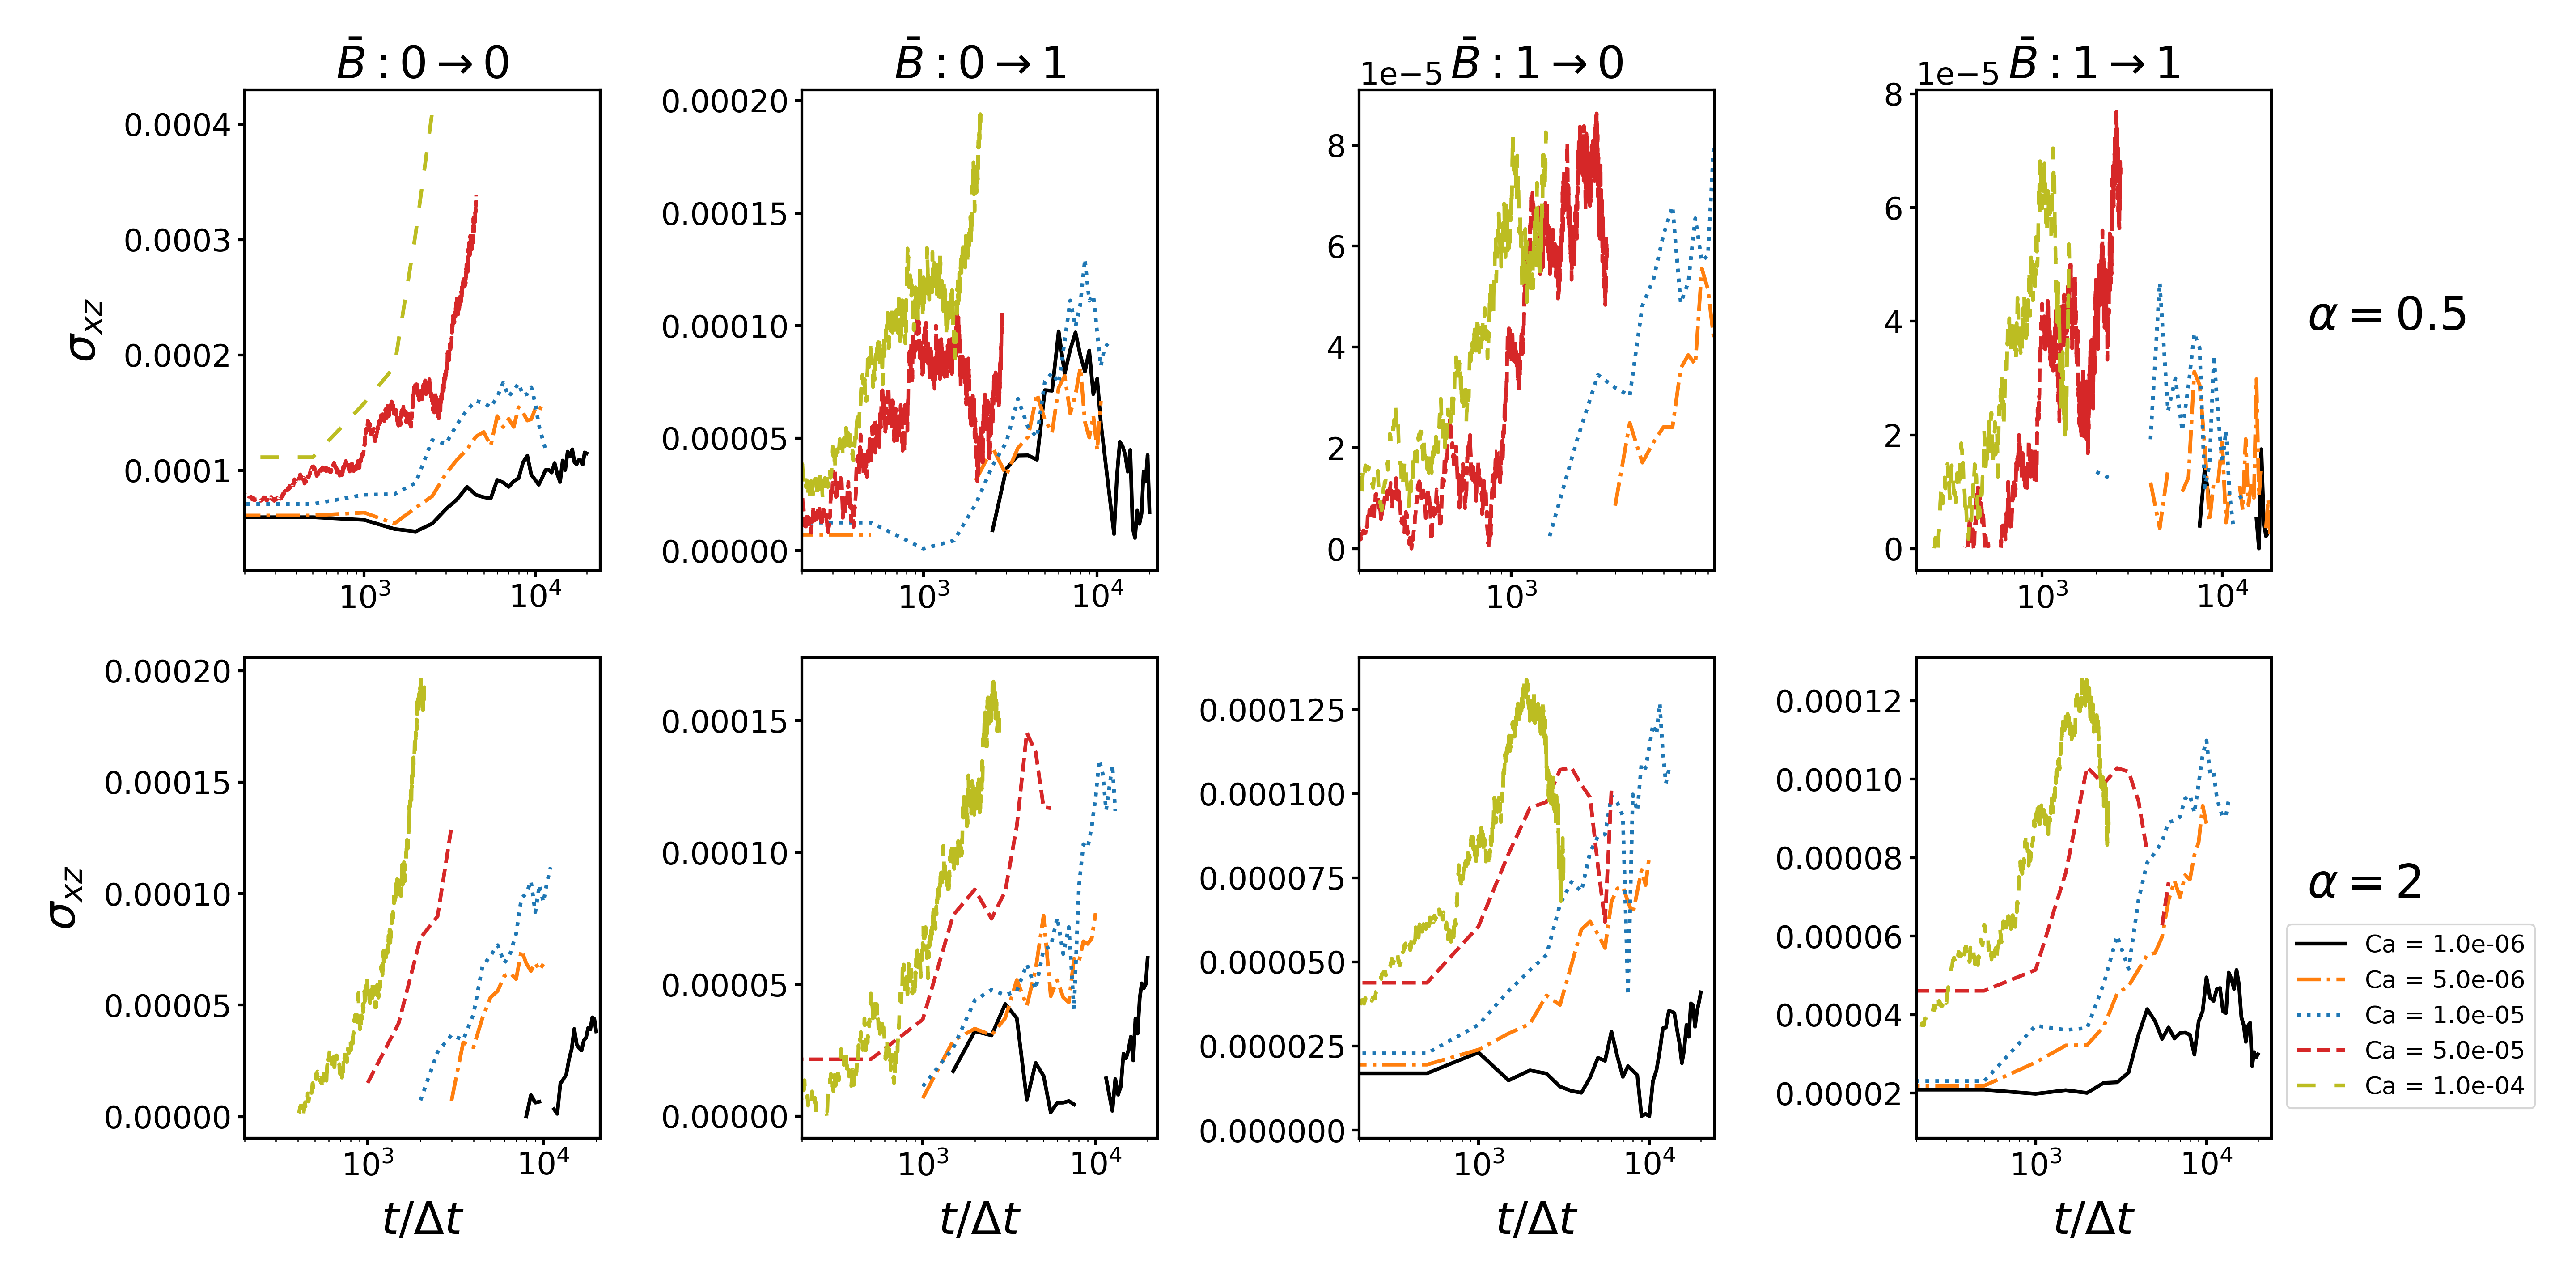
\includegraphics[scale=0.3]{../figures/results/paper3/stress-time_compare.png} 
    \caption{Time evolution of the shear stress of bijels stabilized with ellipsoidal particles as a function of the applied strain rate as
             a function of the initial microstructure and applied magnetic field. The observed stress response is difficult to say when a steady
             state is reached.} 
    \label{fig:stress_time} 
\end{figure}

Figure \ref{fig:stress_time} shows that there is no definitive steady state value of the shear stress obtained in the simulations performed. This is
attributed to the coarsening of the domains and reorientation of particles at the interface. \cite{tavacoli_novel_2011,macmillan_rheological_2019} 
Tavacoli et al. investigated the rheological response of Ethanediol/Nitromethane bijels and identified that upon placement of a needle to calculate the yield
stress of the bijel, the structure of the material was irreversibly altered. \cite{tavacoli_novel_2011} Macmillian et al. identified that repeated 
shearing of a bijel synthesized using direct mixing resulted in degraded mechanical performance. \cite{macmillan_rheological_2019}
To characterize the viscosity, I identify pseudo-steady state regions within each of the shear stress plots and fit the stress identified within this 
pseudo-steady state region to the strain rate. Pseudo-steady state regions are identified by measuring where the rate of change of shear stress is 
smallest for the longest duration. I fit the calculated stress to the applied strain rate using a Herschel-Buckley rheology model defined as
$\sigma_{xz} = \sigma_{y} + K(\dot{\gamma})^{n}$. $\sigma_{xz}$ is the shear stress calculated from the simulation, $\sigma_{y}$ is the yield stress of the bijel, 
$K$ is the flow consistency index and $n$ is the flow index.Where appropriate, I include results corresponding to a shear capillary number of 
$Ca_s = 10^{-6}$ as in many stress responses, $Ca_s = 10^{-6}$ may not always yield usable results. 

\begin{figure} 
    \centering 
    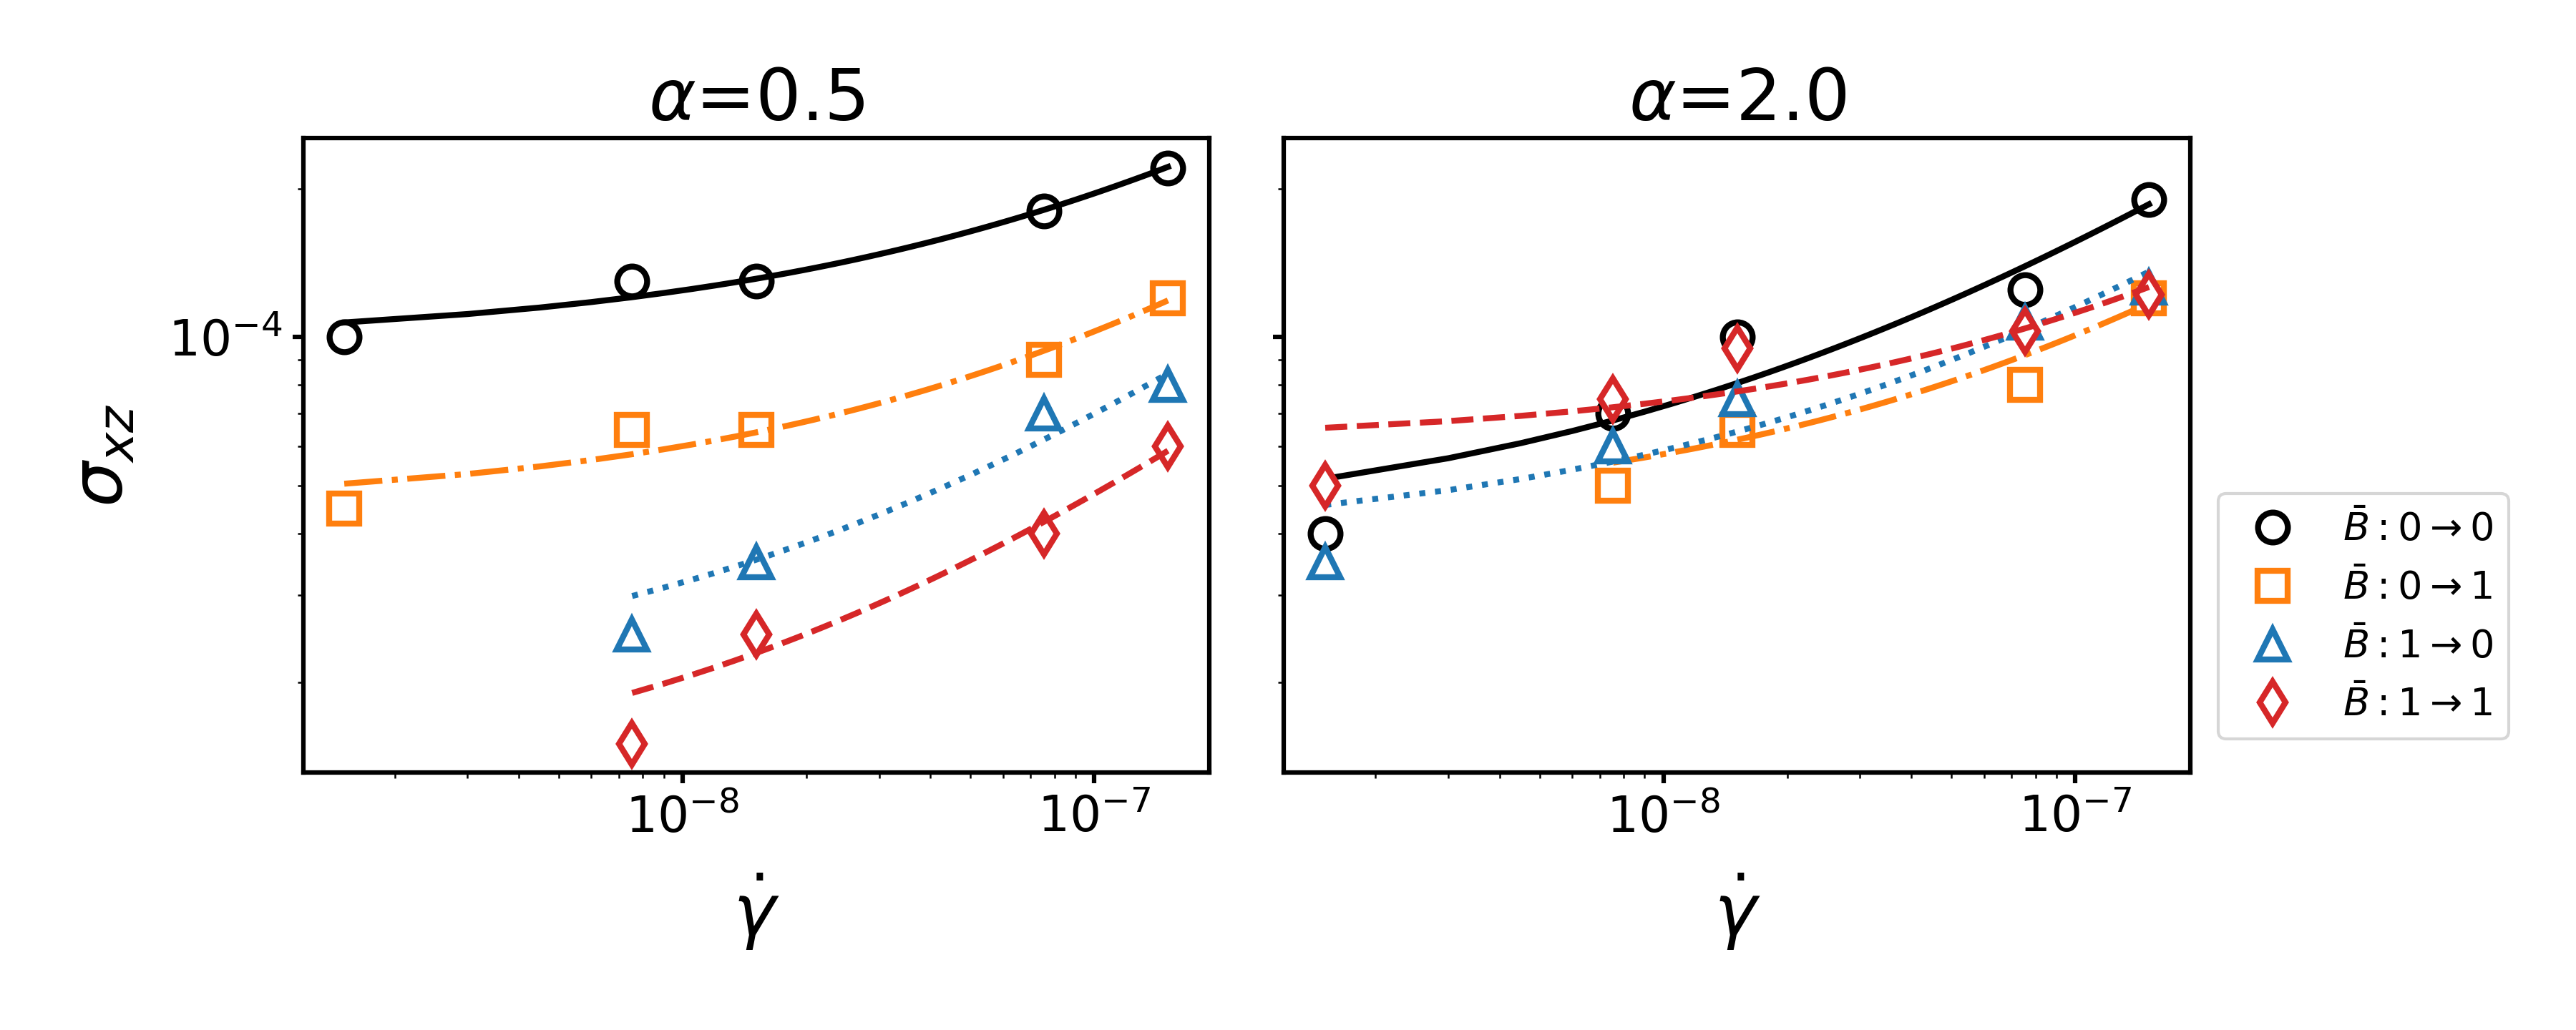
\includegraphics[scale=0.4]{../figures/results/paper3/stress_strain-all.png} 
    \caption{Fitting the experimental shear stress to the strain rate using the Herschel Buckley model. I characterize the bijels are 
             shear thinning in all cases. I show that the bijels become less shear thinning as the particle order increases. I also
             demonstrate that the particle ordering affects the yield stress differently for particles stabilized by oblate and 
             prolate particles.} 
    \label{fig:stress_strain} 
\end{figure}

From Figure \ref{fig:stress_strain}, the slopes of the curve indicate a non-linear shear response to the applied strain rate, suggesting that the rheological properties
are non-Newtonian. Bijels stabilized by prolate and oblate particles also have different shear properties. For bijels stabilized by oblate particles, the stress curves
are more spread out suggesting that there is a larger variance in the properties arising from the change in the initial microstructure of the bijel. From the plot
we can see that the increase in particle order reduces the yield stress of the bijel. For bijels stabilized by rod like particles, the stress response of each processing 
condition is closer together, indicating a smaller variation in the response to the applied magnetic field compared to oblate particles. The shear response upon application
of the magnetic field also suggest that increased ordering of prolate particles makes the bijel more resistant to shear. I quantify the Herschel-Buckley fit parameters and 
tabulate the results in Table \ref{table:rheology_fit}.

\begin{table}[h!]
    \centering
    \begin{tabular}{||c c c c c||} 
     \hline
     Processing & $\alpha$ & $n$ & $K \frac{\Delta m (\Delta t)^{n-2}}{\Delta x} $ & $\sigma_{y} \frac{\Delta m}{\Delta x (\Delta t)^2}$ \\ [0.5ex] 
     \hline\hline
     $\bar{B}: 0 \rightarrow 0$ & 0.5 & 0.511 & 0.999 & $7.168 \cdot 10^{-5}$ \\ 
     \hline
     $\bar{B}: 0 \rightarrow 1$ & 0.5 & 0.579 & 0.944 & $4.008 \cdot 10^{-5}$ \\
     \hline
     $\bar{B}: 1 \rightarrow 0$ & 0.5 & 0.642 & 0.888 & $4.945 \cdot 10^{-5}$ \\
     \hline
     $\bar{B}: 1 \rightarrow 1$ & 0.5 & 0.637 & 0.914 & $1.715 \cdot 10^{-5}$ \\
     \hline
     $\bar{B}: 0 \rightarrow 0$ & 2 & 0.561 & 0.965 & $4.618 \cdot 10^{-5}$ \\
     \hline
     $\bar{B}: 0 \rightarrow 1$ & 2 & 0.609 & 0.944 & $4.101 \cdot 10^{-5}$ \\
     \hline
     $\bar{B}: 1 \rightarrow 0$ & 2 & 0.597 & 0.899 & $5.025 \cdot 10^{-5}$ \\
     \hline
     $\bar{B}: 1 \rightarrow 1$ & 2 & 0.606 & 0.885 & $6.435 \cdot 10^{-5}$ \\ [1ex] 
     \hline
    \end{tabular}
    \caption{Hershel Buckley fit parameters for different processing conditions applied to bijels stabilized by ellipsoidal particles.}
    \label{table:rheology_fit}
\end{table}
 
The results in Table \ref{table:rheology_fit} show that bijels remain shear thinning regardless of the processing history and particle morphology.
The particle morphology dependent differences in the shear response characterized in Figure \ref{fig:stress_strain} are quantified in Table \ref{table:rheology_fit}
where the yield stress differences predicted is clear to see. I also show that bijel templates with an applied field of $\bar{B} = 1$ have larger flow indices \
than bijel templates made with no applied field. The same trend exists here where the application of a magnetic field makes the bijel more Newtonian. I also 
characterize that the yield stress of bijels stabilized with oblate particles decrease as the initial order of the particles and the applied field onto the bijel increase. 
The yield stress of bijels stabilized by prolate particles increases as the initial order of the particles and the applied field onto the bijel increase. In previous aims, I 
characterized that application of magnetic fields created orientational ordering of the bijels and that the local ordering of the bijels change. I 
showed that as magnetic fields were applied, oblate particles have lower local ordering on the interface while for prolate particles it increases.
Past investigations have identified that particle monolayers buckle more easily as local particle ordering decreases. \cite{prakash_buckling_2024} 
They identified that local ordering can enhance stress distribution among particles, making locally ordered particle monolayers better at withstanding shear.
I visualize the ordering of the particles at the interface to the z direction for both particle morphologies at $Ca_s = 10^{-6}$ for the 
case $\bar{B}: 1 \rightarrow 0$.

\begin{figure} 
    \centering 
    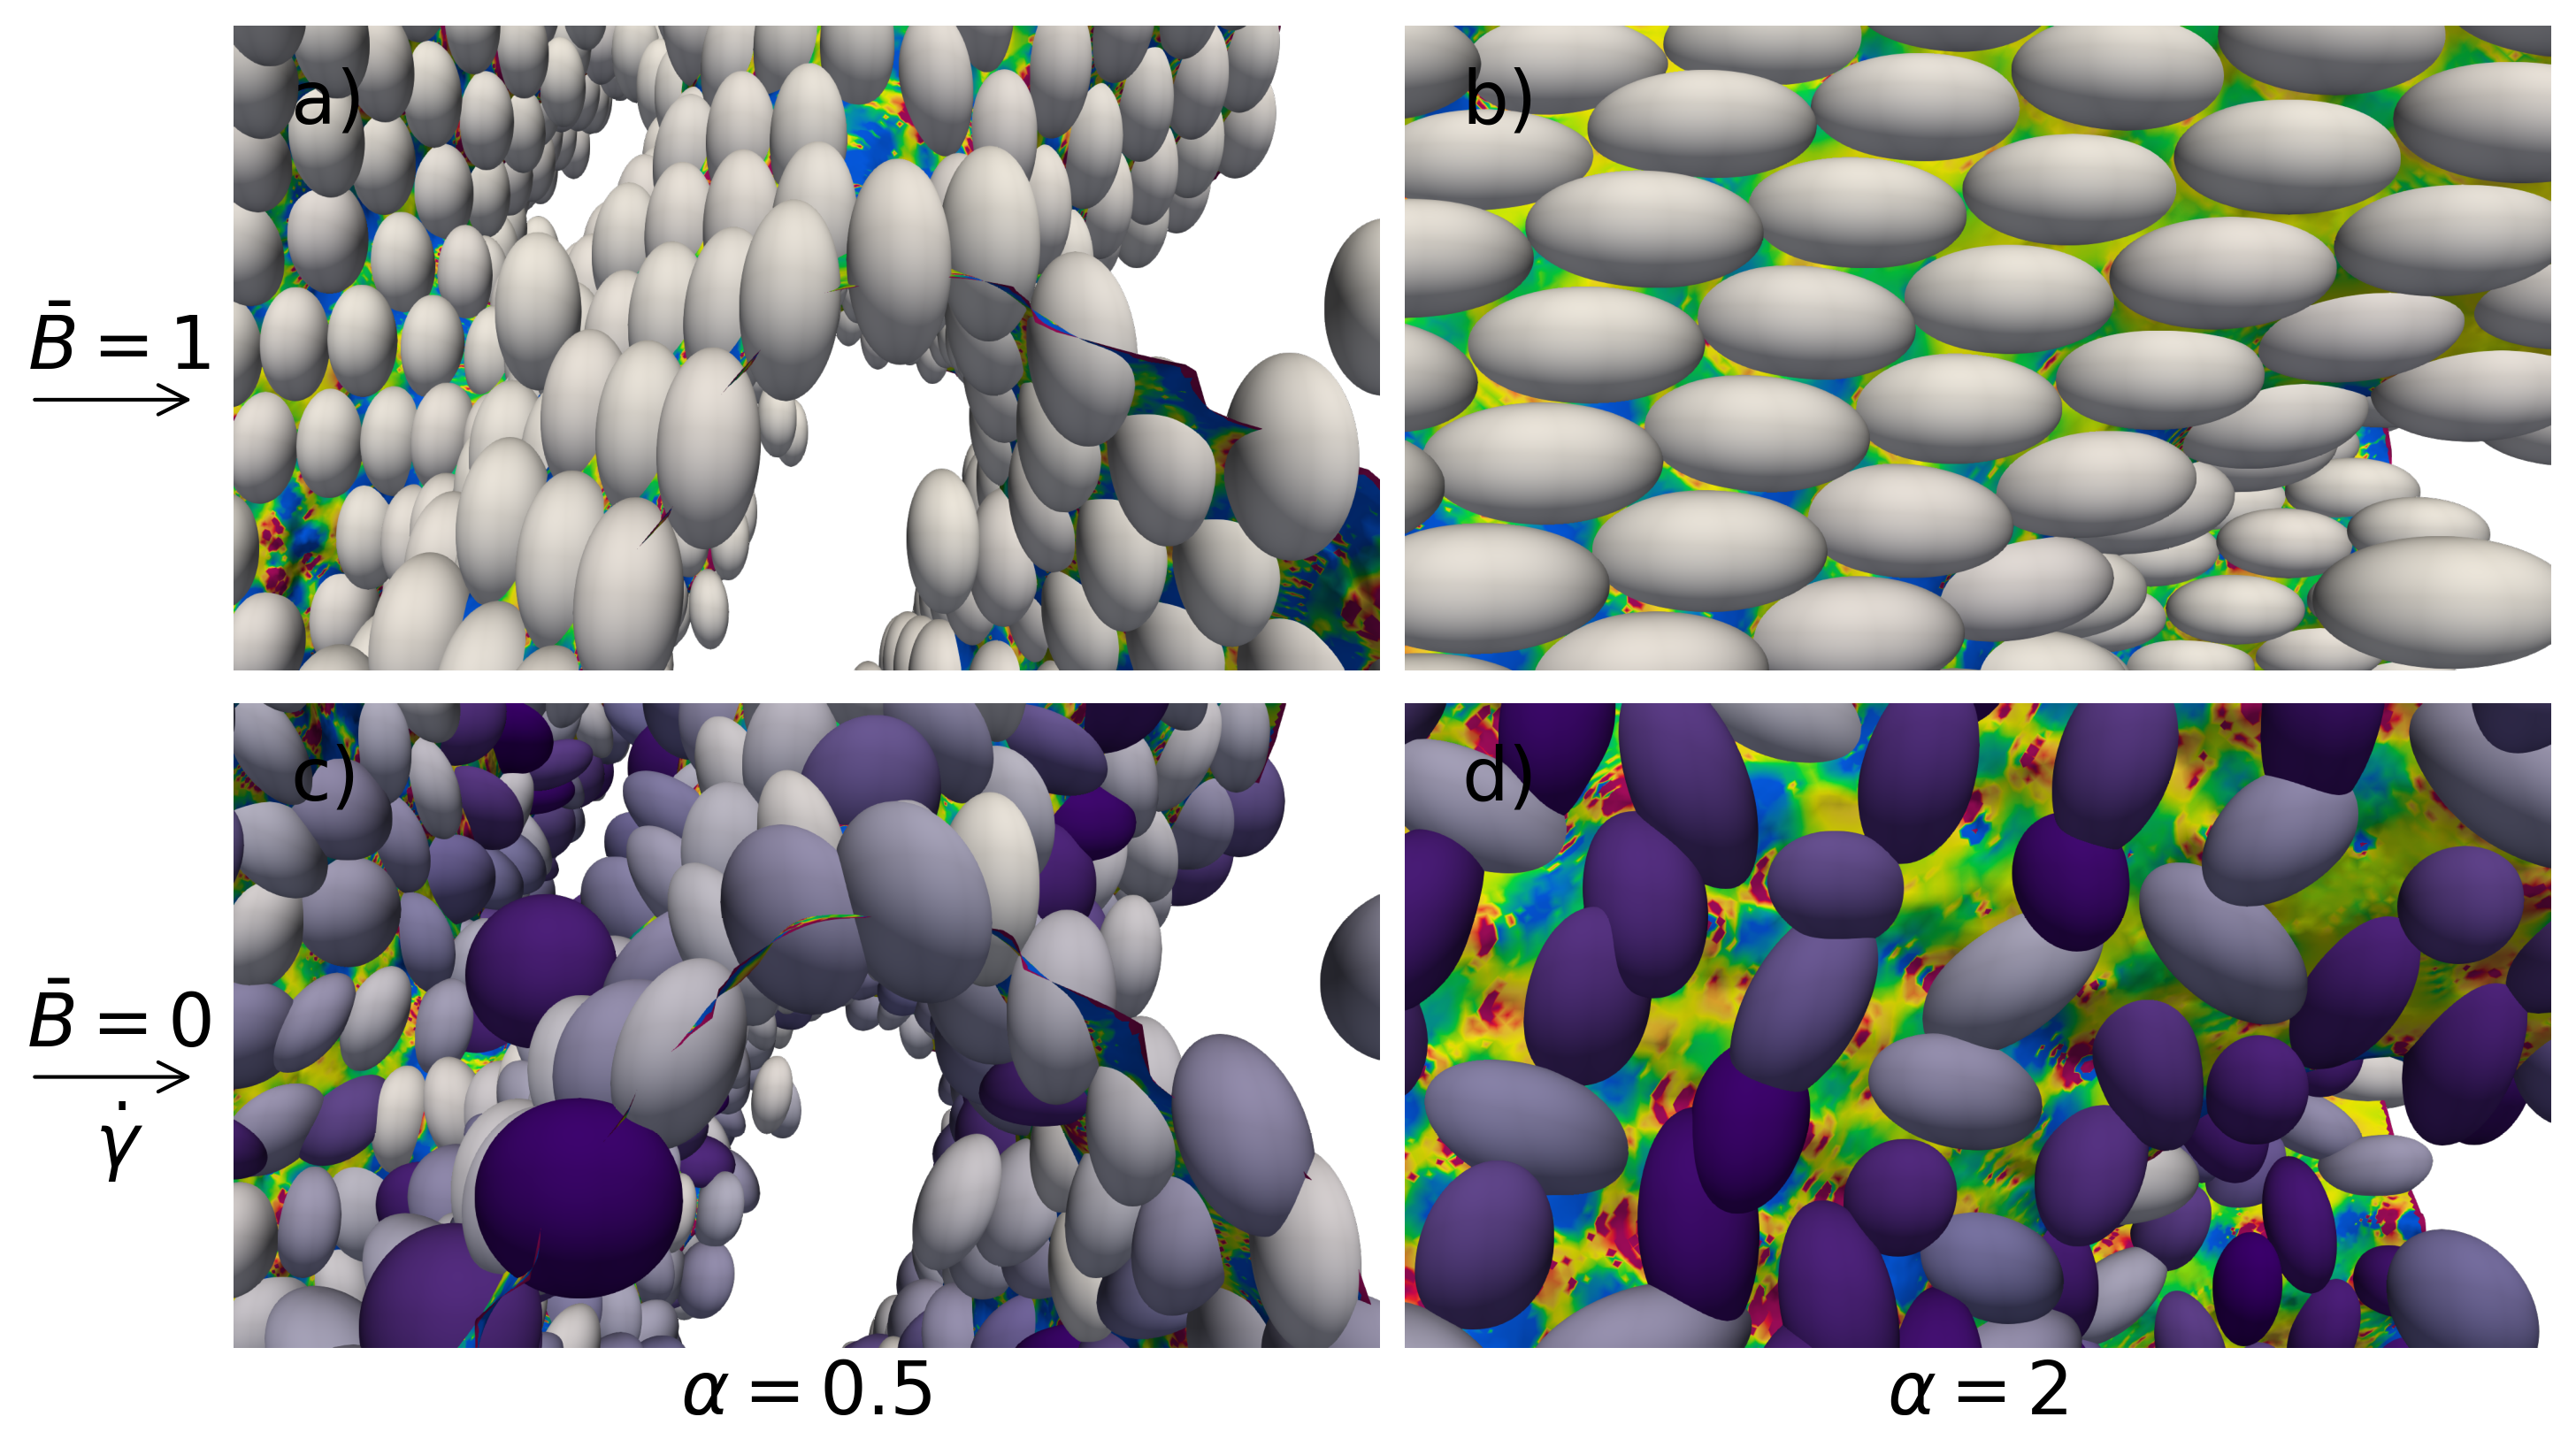
\includegraphics[scale=0.4]{../figures/results/paper3/tz_concat_startB-1_endB-0.png} 
    \caption{Visualization of the particle monolayer of bijels stabilized by prolate and oblate ellipsoidal particles with processing history $\bar{B}: 1 \rightarrow 0$
             undergoing an applied shear of $Ca_s = 10^{-6}$. Particles with a deeper purple shade have a larger angle to the z axis. The top row shows the initial 
             configuration of the particles while the bottom row shows the final configuration of the particles. } 
    \label{fig:particle_viz_tz} 
\end{figure}

In Figure \ref{fig:particle_viz_tz}, the particles are initially ordered to the direction of the applied magnetic field. Upon application of shear and removal
of the magnetic field, I see that the particles begin reorienting away from the z direction. I also observe that the reorientation of particles uncovers the interface.
The reorientation observed is particle morphology specific with prolate particles seeing more reorientation away from the applied shear direction than oblate particles.
Looking at the images, I see that prolate particles rotate away from the direction of the magnetic field and applied shear towards the direction of the shear gradient,
while oblate particles reorient towards minimizing area to the applied shear direction. While these snapshots show the initial and final orientations of the particles at the
interface, we can characterize the time evolution of the particle monolayer changes to identify its role in the rheological properties characterized.

\subsection{Particle properties}

Particles at the interface of bijels stabilized with ellipsoidal particles reorient at the interface to minimize interfacial and
steric energies. \cite{gunther_timescales_2014} The particles stabilizing bijels in confined systems under shear have been shown to
orient to the direction of shear and ejected from the interface at sufficiently long times or shear.\cite{bonaccorso_shear_2020} 
I probe these aspects of the particle monolayer in this section. I plot the orientation of the particle to each cartesian axis 
to identify if I characterize shear induced ordering.

\begin{figure} 
    \centering 
    \includegraphics[scale=0.3]{../figures/results/paper3/angle_to_cartesian-SS.png} 
    \caption{Comparisons of the initial and final particle orientations of the particles to each cartesian direction under
             four processing histories for bijels stabilized with oblate and prolate ellipsoids at multiple shear rates. I show
             shear dependent ordering of the particle monolayer if the initial particle monolayer begins with particle order.} 
    \label{fig:particle_orientation_cartesian_shear} 
\end{figure}

From Figure \ref{fig:particle_orientation_cartesian_shear} I see that with bijel templates simulated under $\bar{B} = 0$, the
particles adopt a random orientation. Upon application of shear, I see that there is little directional ordering to the 
shear direction in the simulation time observed. Upon application of the magnetic field in the $\bar{B}:0 \rightarrow 1$ case, 
the particles order to the direction of the magnetic field. Here we see that the prolate particles order more readily to the applied
field than the oblate particles, seen as a larger clustering of particles at the $\theta_z = 0$ corner of the triangle. In the 
$\bar{B}:1 \rightarrow 0$ case particle morphology dependent partial relaxation of the particles away from the magnetic field direction 
is observed. Directionality of the particles to the field is still observed, suggesting that the ordering of the particles is not
immediately removed once the field is switched off. In the processing history of $\bar{B}:1 \rightarrow 1$, particles are locked
into ordering to the magnetic field direction. However we also see that some particles are reoriented away from the field direction
due to the applied shear. Prolate particles have a smaller distribution of particle orientations than oblate particles, suggesting that
the initial orientation and ordering of particles to the shear applied underpin the response observed. As the particles are adsorbed on the 
interface, the orientation of the particles are influenced by a balance between magnetic forces from the field and capillary forces 
from the interface. We can qualitatively calculate the time evolution of the capillary interactions using the interfacial angle.

\begin{figure} 
    \centering 
    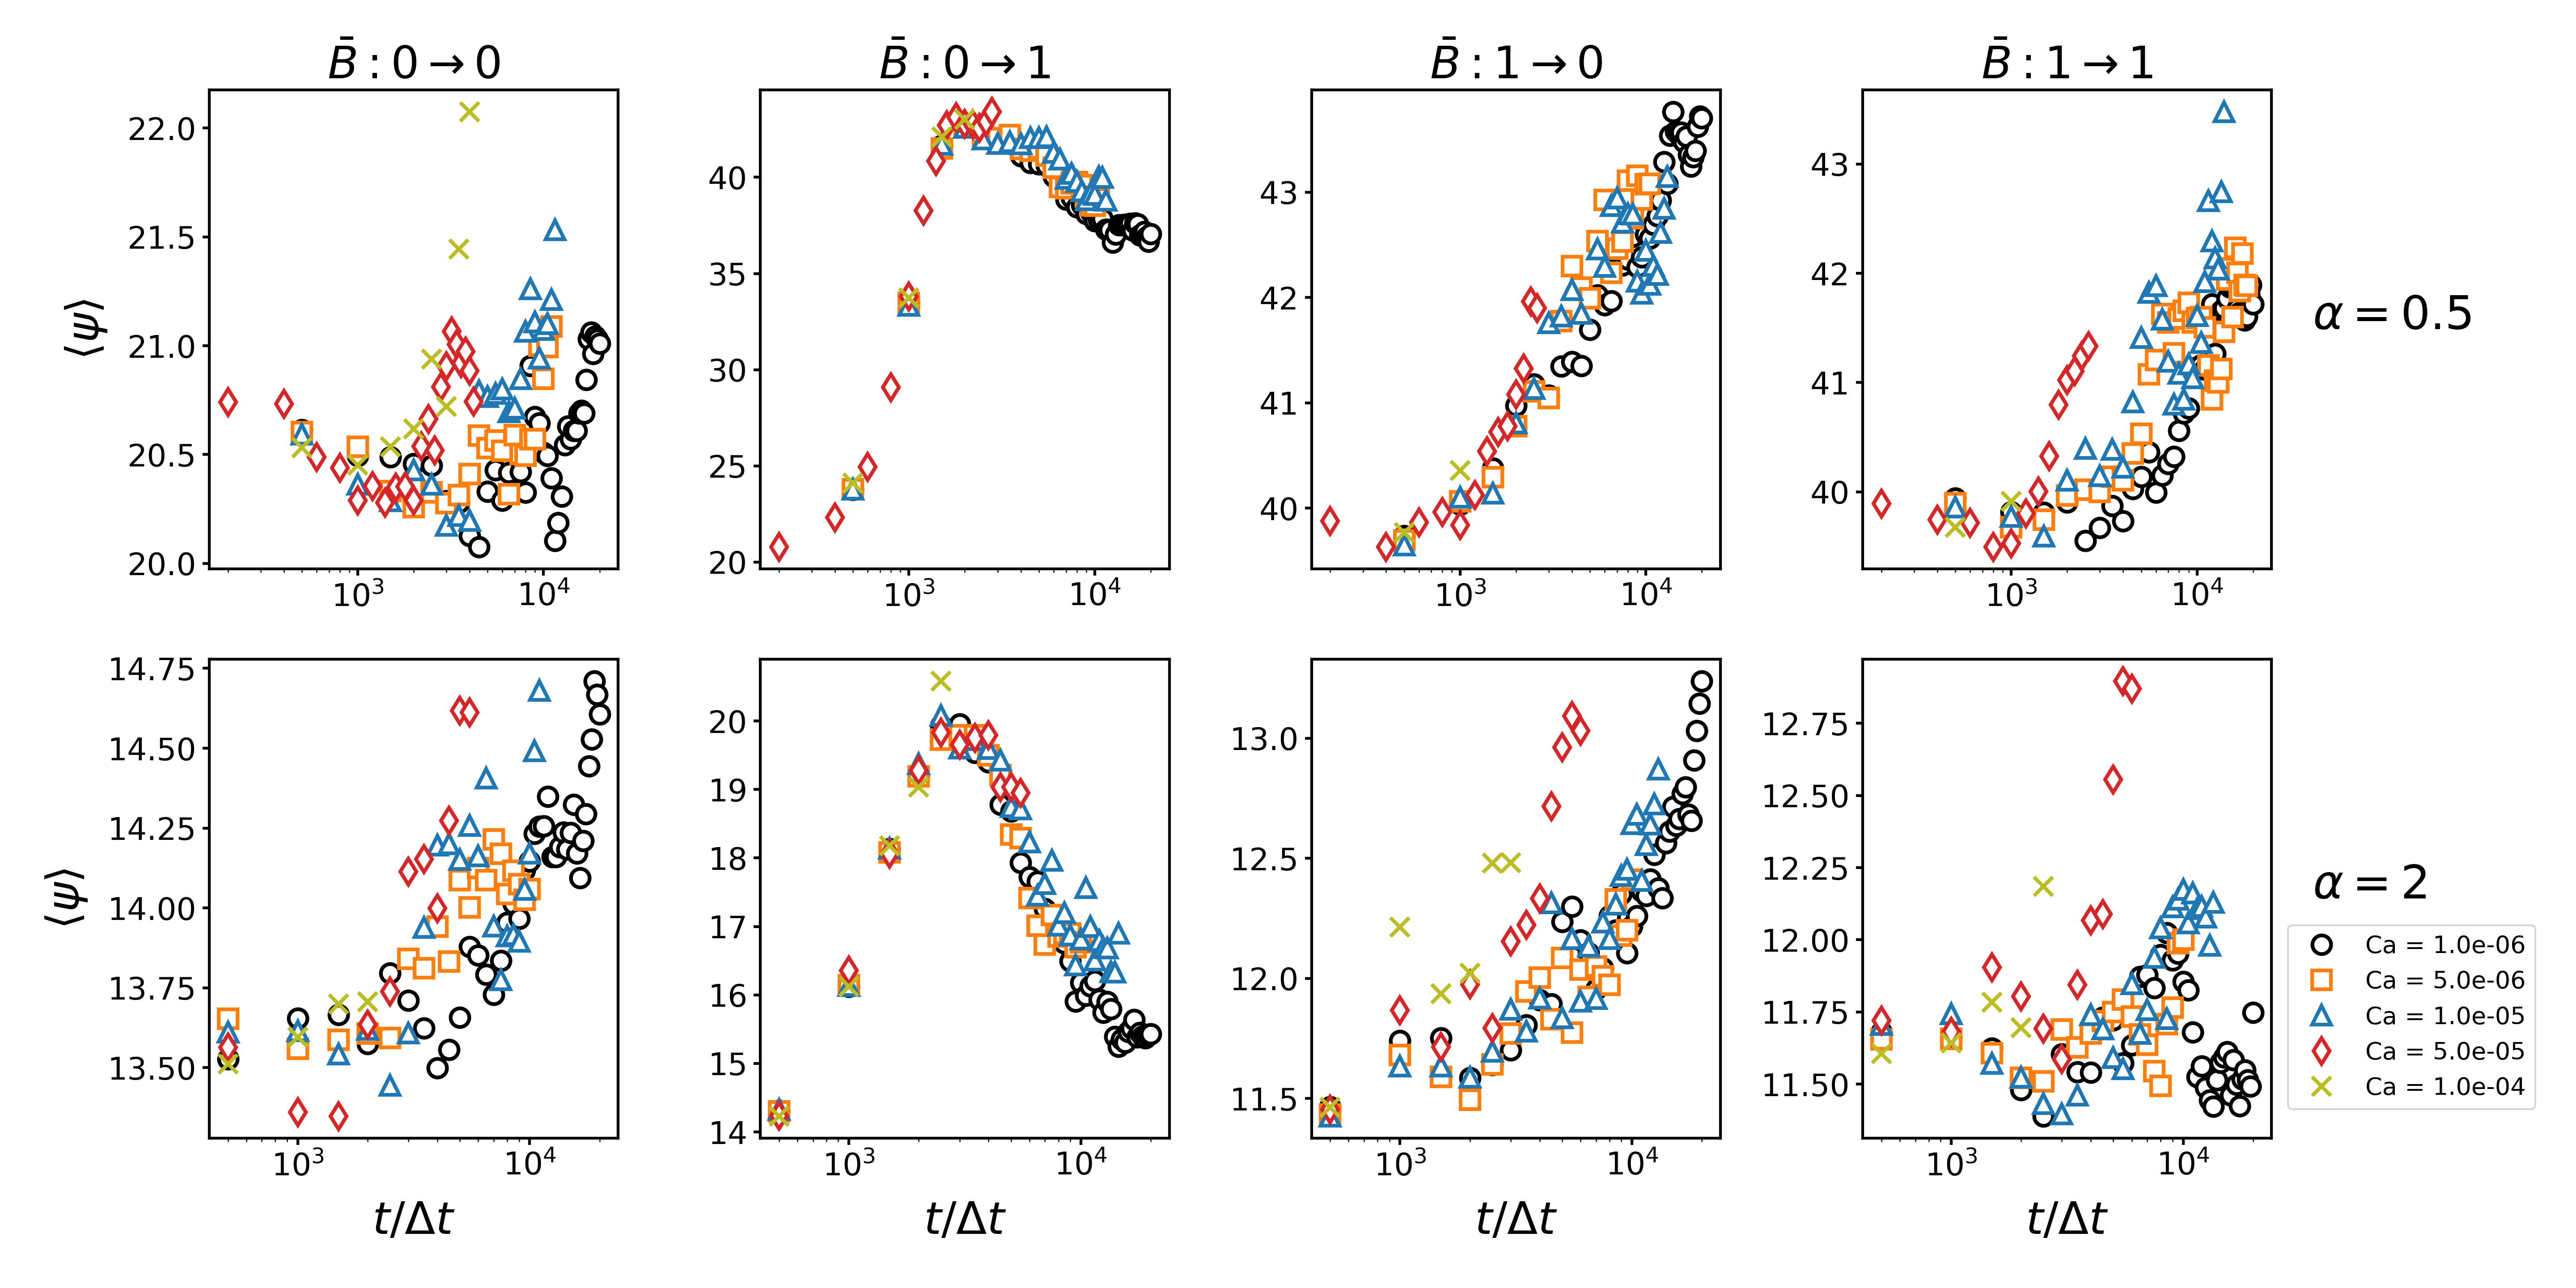
\includegraphics[scale=0.3]{../figures/results/paper3/psi-time_compare.png} 
    \caption{Comparisons of the interfacial angle of bijels stabilized by ellipsoidal particles as a function of 
             the applied shear rate at four different processing histories. I show that upon application of shear
             particles tilt out of the interface reduces the interfacial area stabilized. $\bar{B}: 0 \to 1$ shows 
             large variations in the interface angle.} 
    \label{fig:interface_angle_shear} 
\end{figure}

From Figure \ref{fig:interface_angle_shear}, I demonstrate that there is a slow increase in the interface angle over time for all cases
except for $\bar{B}: 0 \to 1$. For the $\bar{B}: 0 \to 1$ case, this has been shown in Chapter \ref{chapter:aim2} to be due to particle
reorientation to the applied magnetic field. For all other cases, we see an average increase in $\langle \psi \rangle$ over time, showing
that the particles under shear reorient out of the interface. Particles reorienting out of the interface can be due to shear induced interfacial 
stress, modifying the curvature of the interface and thus the lowest energy particle orientation to the interface or shear induced increases in
interparticle forces, causing the particle to tilt out of the interface to minimize interparticle forces. We can characterize the latter 
mechanism through measurements of the number of particles on the interface as increases in interparticle forces result in ejection of
particles from the interface. 

% We can characterize the impact of the interfacial angle on the 
% particle packing using the radial distribution function (rdf).

% \begin{figure} 
%     \centering 
%     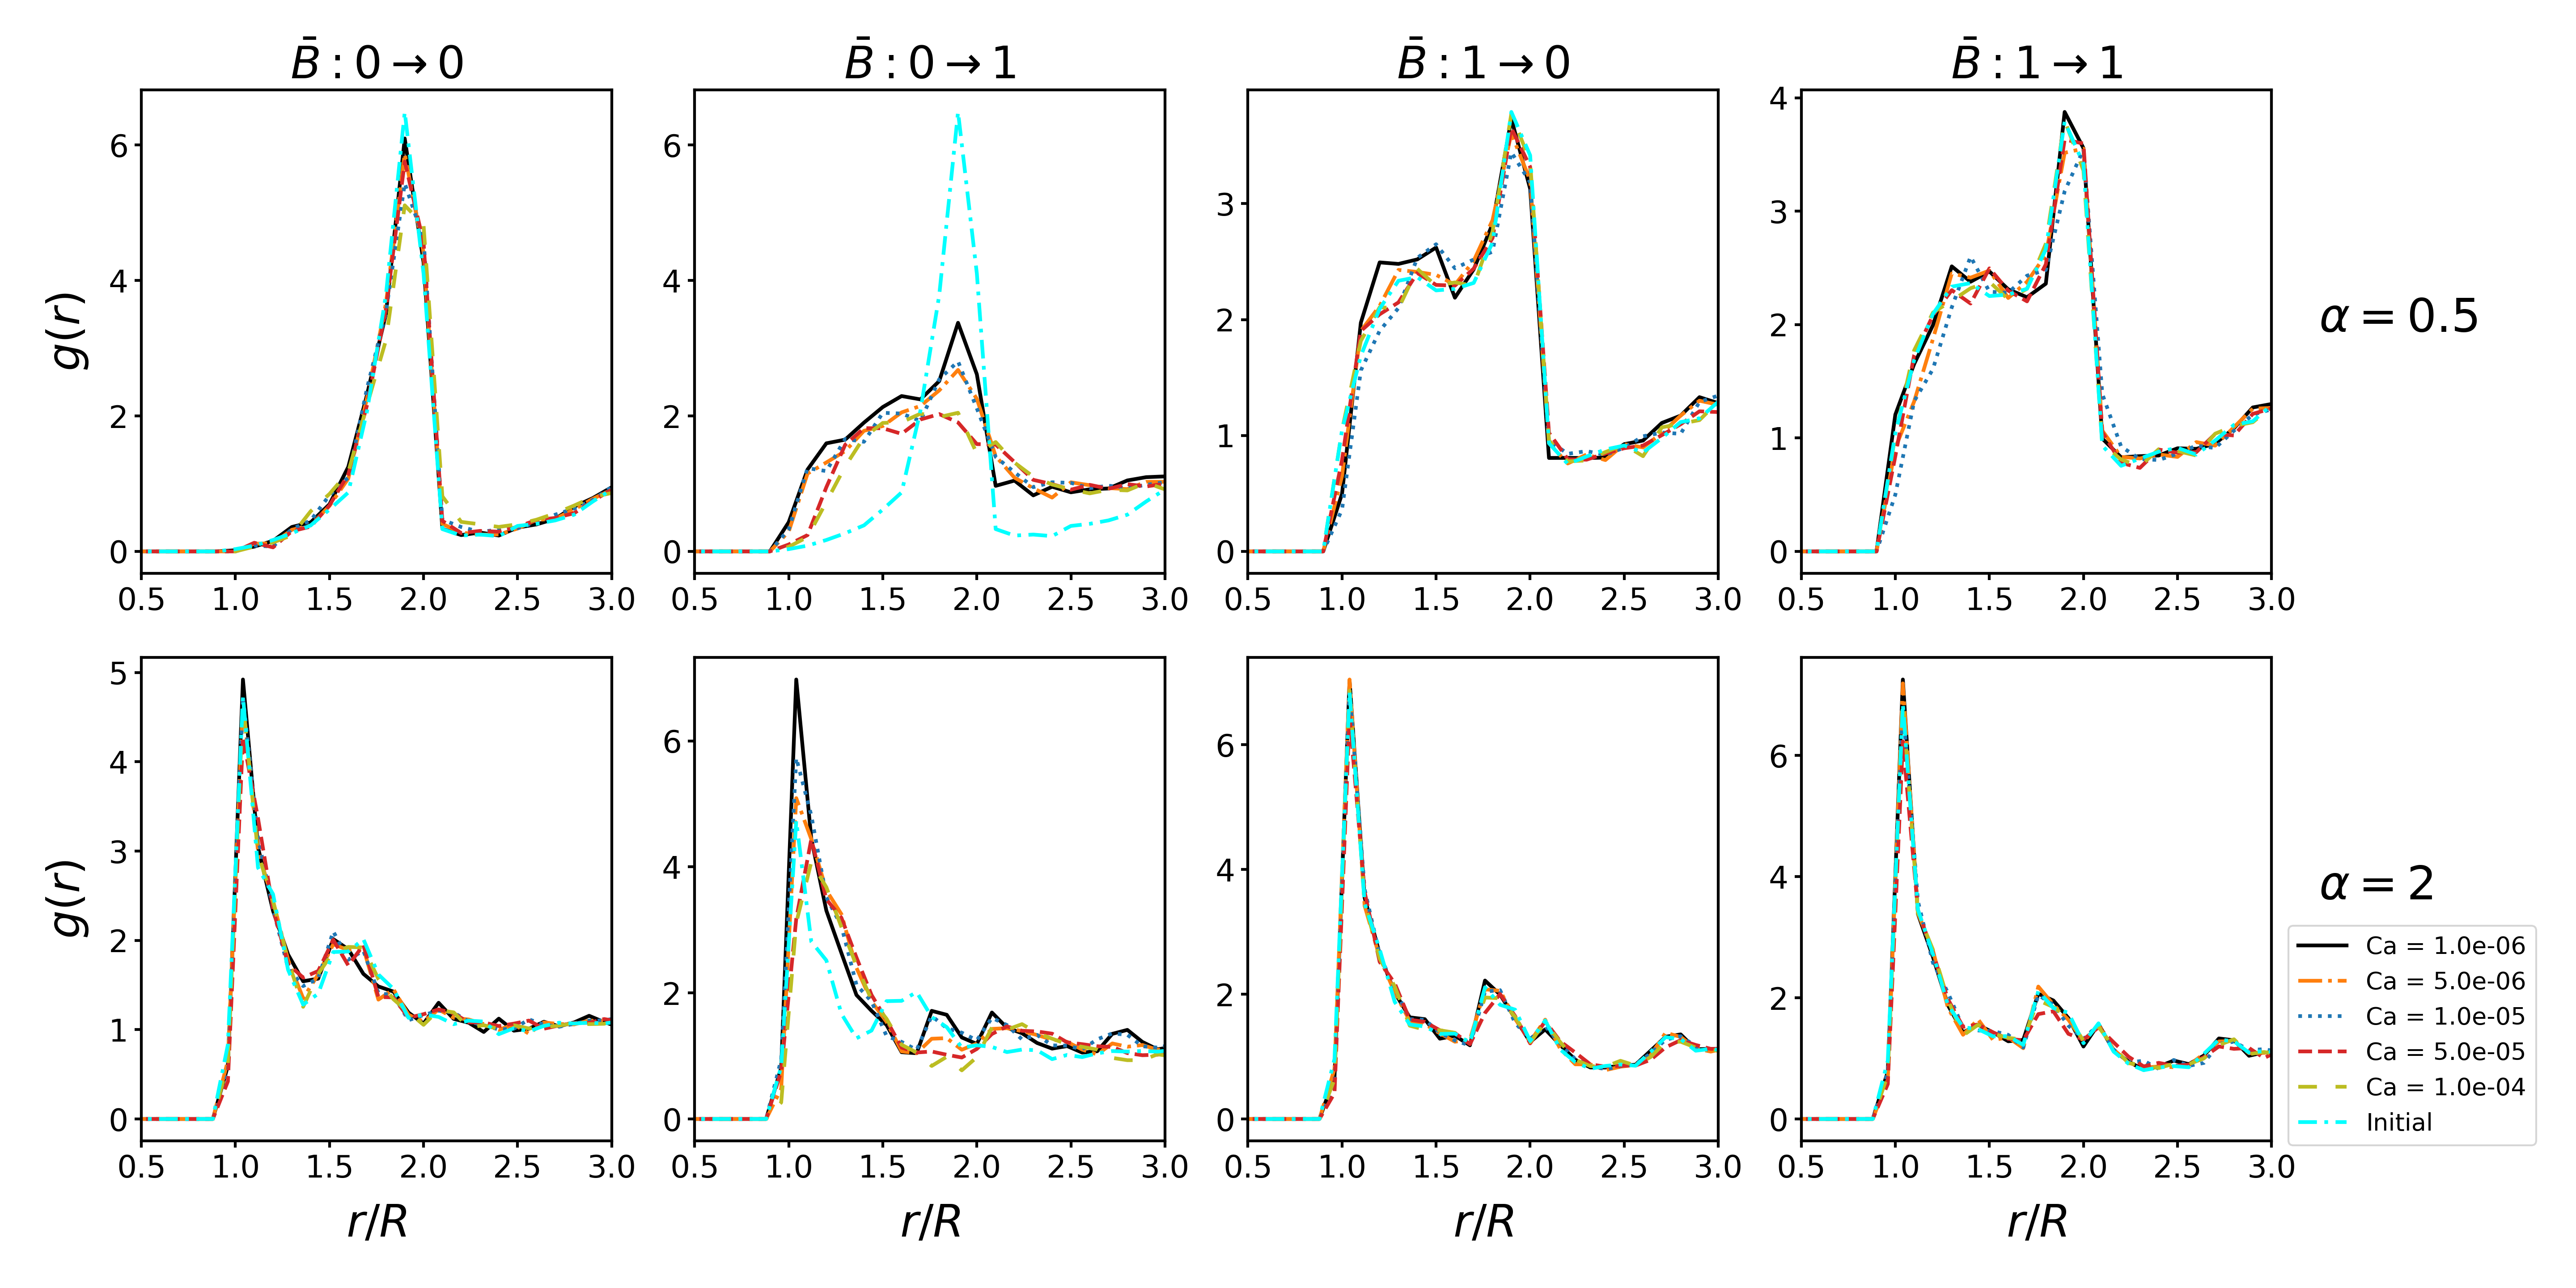
\includegraphics[scale=0.3]{../figures/results/paper3/rdf-SS.png} 
%     \caption{Comparisons of the initial and final radial distribution function of the particles of bijels stabilized by ellipsoidal 
%     particles as a function of the applied shear rate at four different processing histories. I show that there are minor differences
%     in the particle ordering at the interface, suggesting that the particle tilting affects the coverage of particles at the interface.} 
%     \label{fig:rdf_shear} 
% \end{figure}

% From Figure \ref{fig:rdf_shear}, I show that the change in the packing of the particles on the interface is not correlated to the change 
% in the interfacial angle of the particles on the interface when changing the applied field strength in all cases. I then characterize the proportion 
% of particles on the interface to investigate how the proportion of particles on the interface changes and its impact on the interfacial area.

\begin{figure} 
    \centering 
    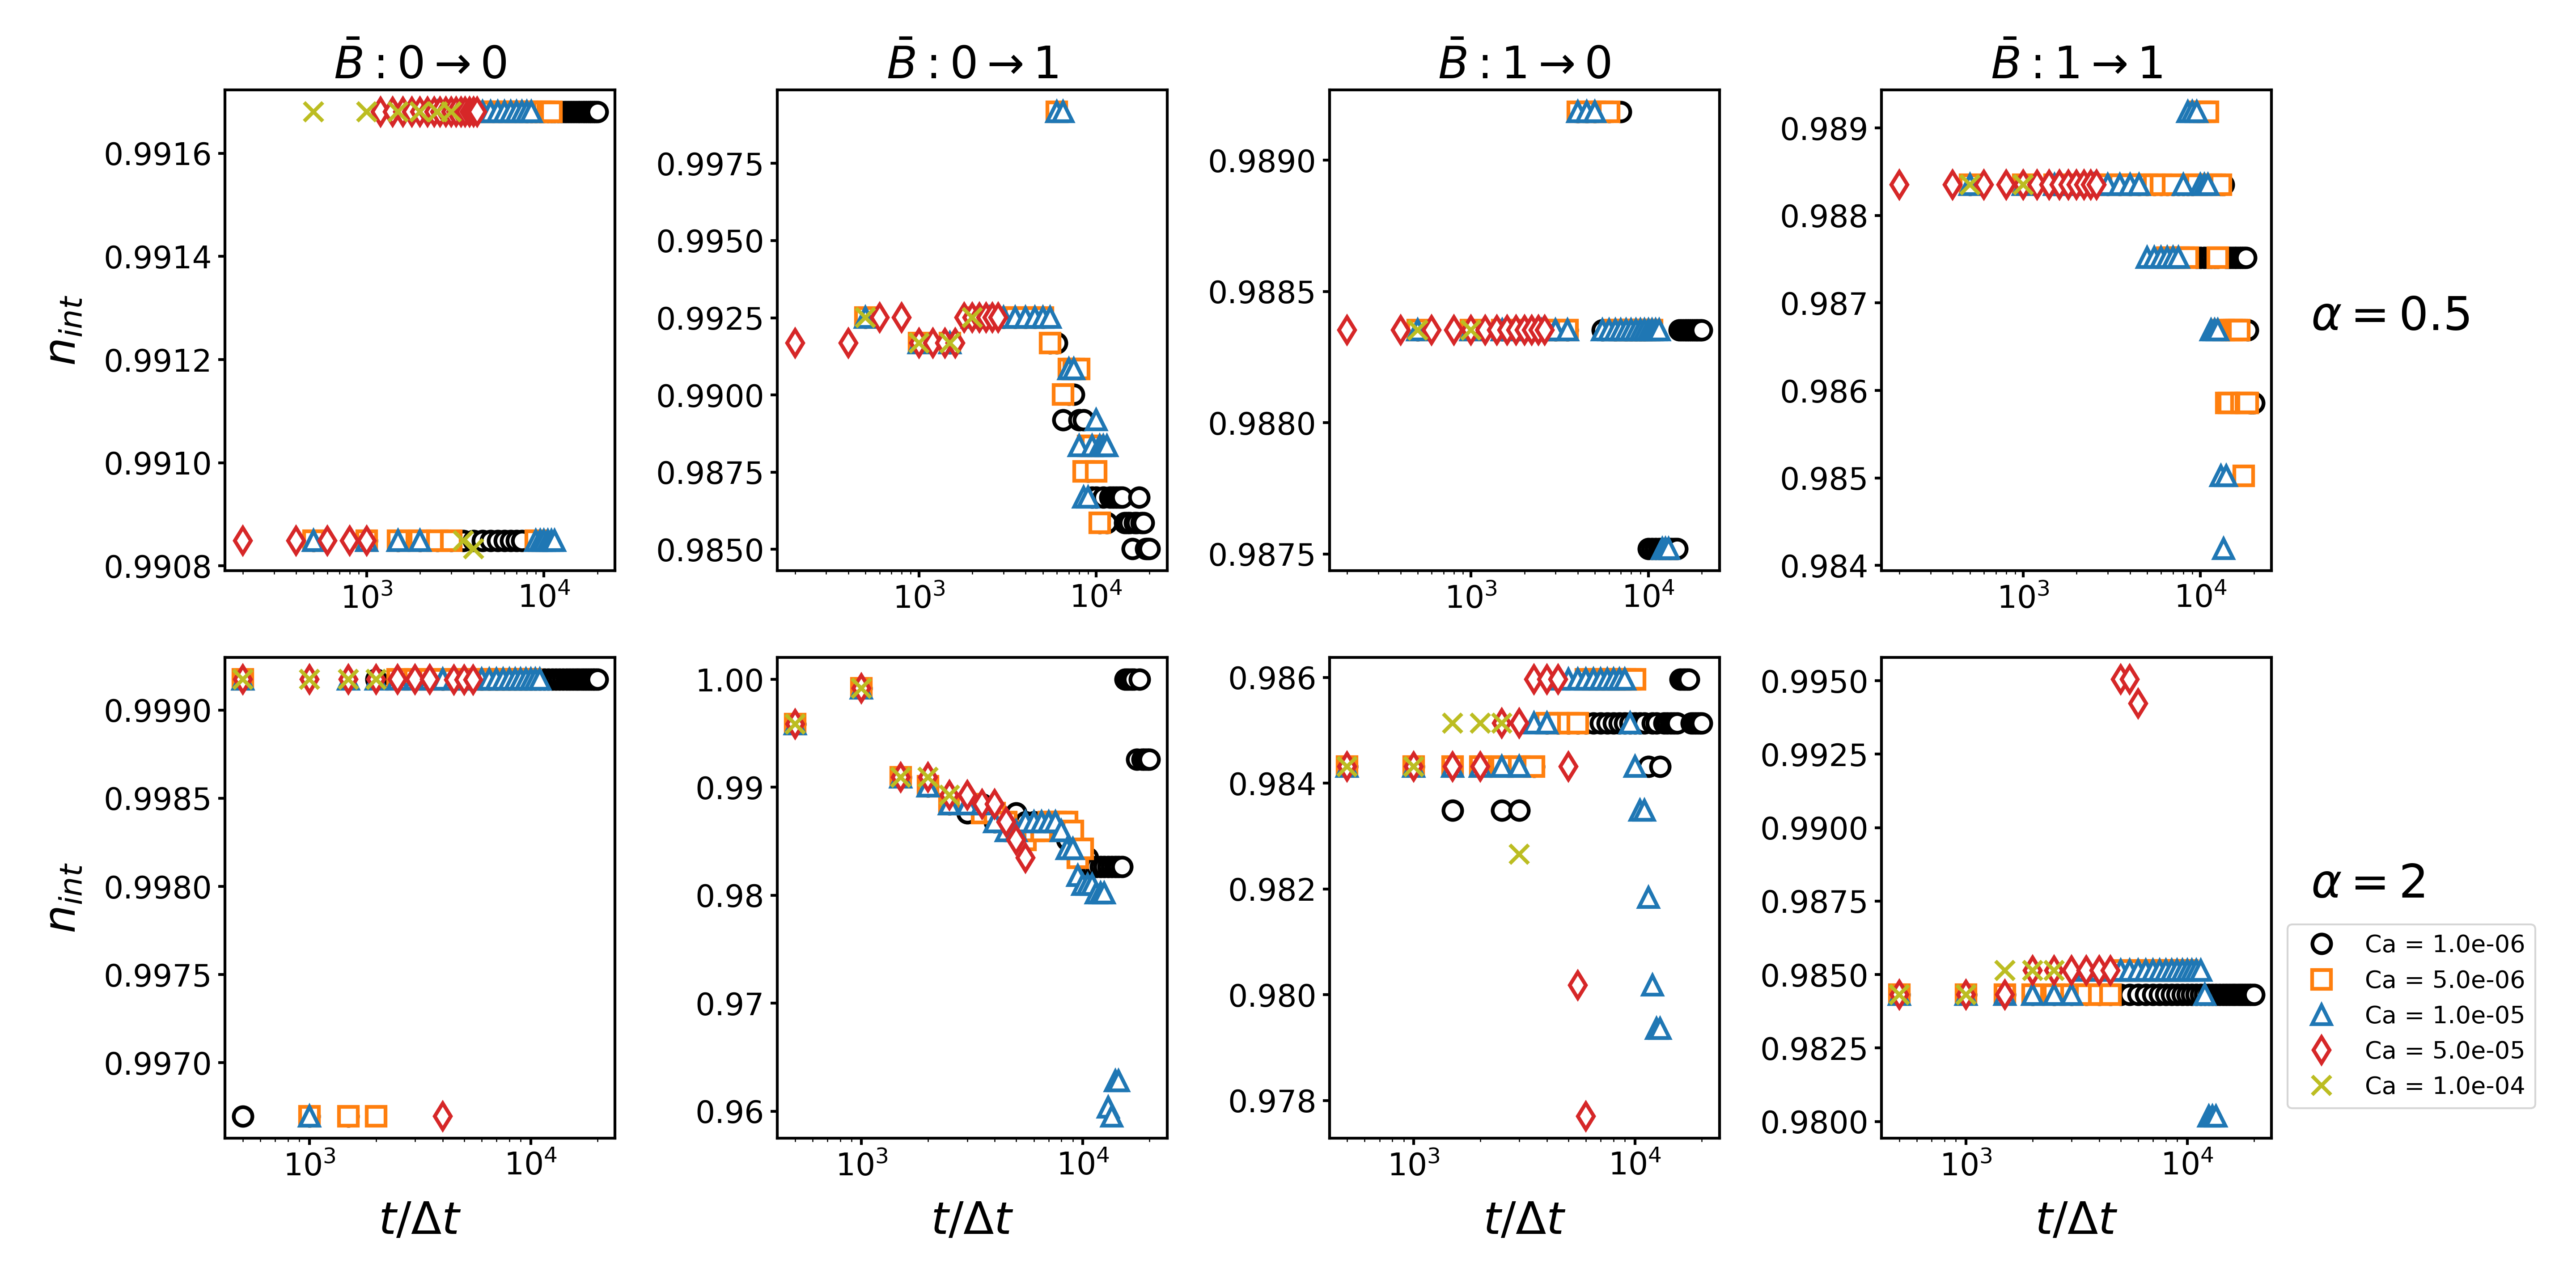
\includegraphics[scale=0.3]{../figures/results/paper3/n_int-time_compare.png} 
    \caption{Comparisons of the proportion of particles on the interface of bijels ($n_{int}$) stabilized by ellipsoidal particles as a function of 
             the applied shear rate at four different processing histories. I show that upon application of shear, many cases have a 
             reduction in the number of particles on the interface while in others it stays the same. For cases where $n_{int}$ reduces, I can 
             attribute the domain size coarsening to this effect.} 
    \label{fig:particles_interface_prop_shear} 
\end{figure}

I show in Figure \ref{fig:particles_interface_prop_shear} that when the magnetic field is kept the same between the template and during shear, the
proportion of particles on the interface ($n_{int}$) stays approximately the same. However when changing the applied field strength, $n_{int}$ more 
sensitive to shear. Here I also characterize that increasing the applied field strength reduces $n_{int}$ more than decreasing it. To characterize 
the role of the interface properties and the impact of particle ejection and tilting of particles out of the interface,the next section aims to 
uncover the microstructural implications of these effects.

% This is consistent
% with the amount of coarsening observed for each case seen in Figure \ref{fig:domain_size_time_shear} where $\bar{B}:0 \rightarrow 1$ shows the largest
% change.

\subsection{Microstructure change}

Bonaccorso et al. identified that the spherical particle stabilizers in their bijel simulations oriented to the direction of shear before being
ejected from the interface. \cite{bonaccorso_shear_2020} This then led to the domains of the bijel to coalesce and eventually destruction of the
bicontinuous microstructure. \cite{bonaccorso_shear_2020} In our bijels, we also characterize this behavior upon application of shear.
In this section, I probe the effect of applied shear to the microstructure of magnetically
responsive bijels stabilized by ellipsoidal particles. To investigate the effect of the particle angle on the interfacial coverage of the bijel,
I plot the area averaged gaussian curvature over time. This parameter will allow insight into the evolution of the interface, namely the presence of
domain coarsening, coalscence or break-off events.

\begin{figure} 
    \centering 
    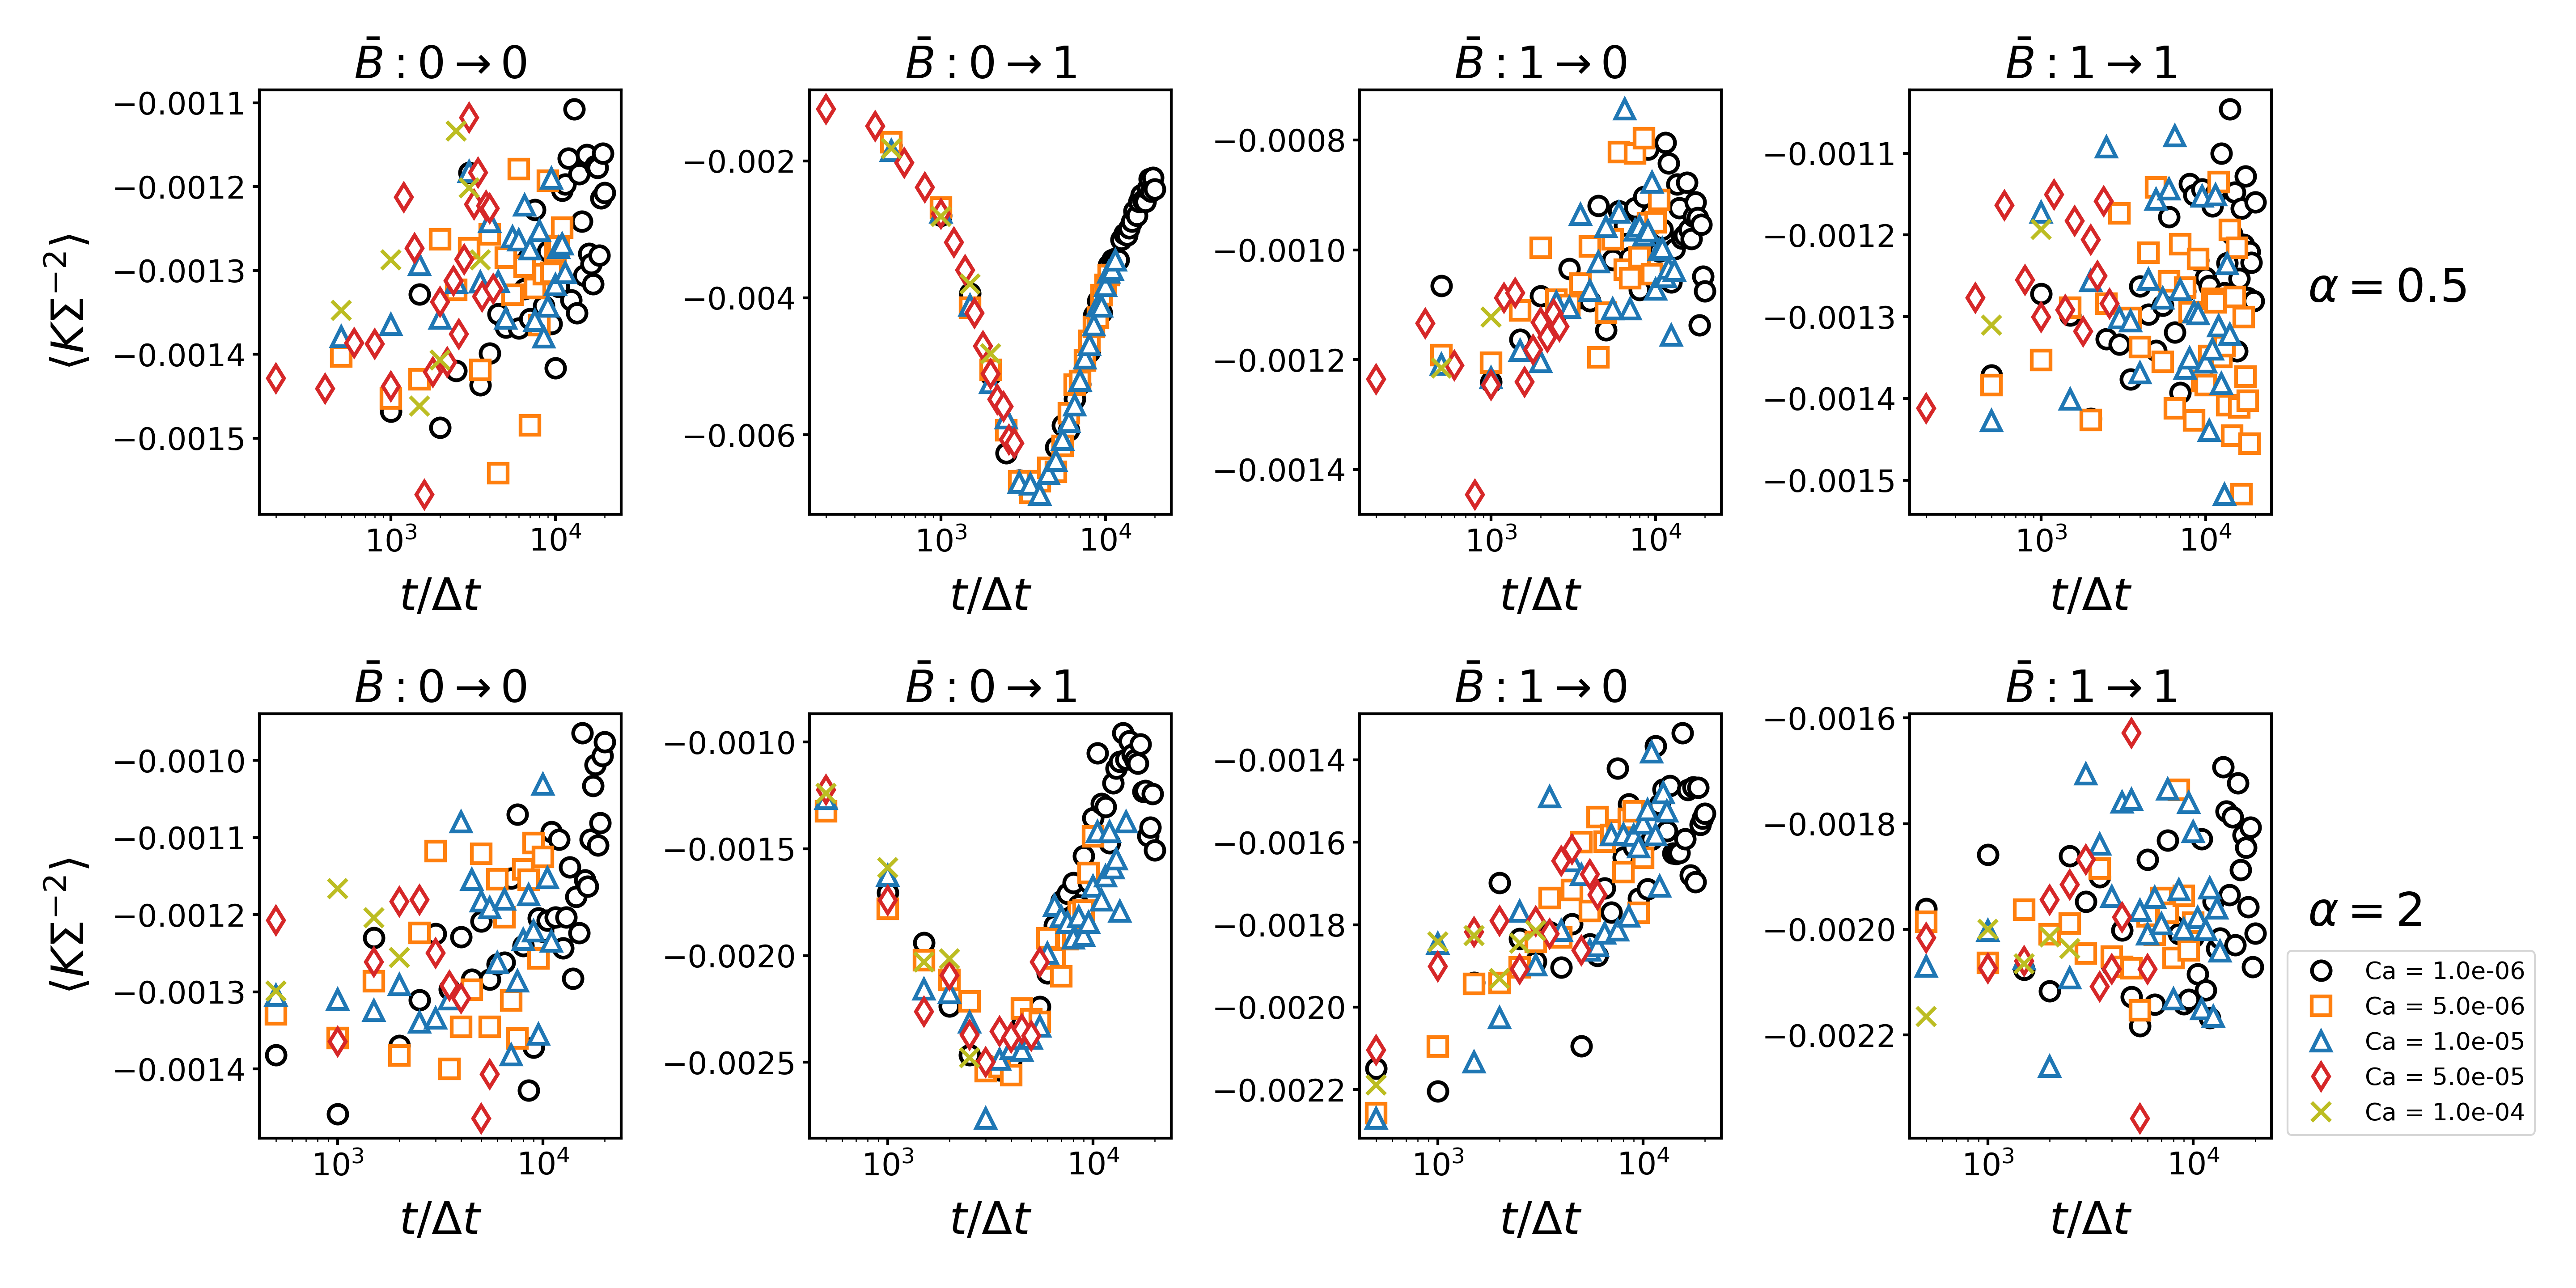
\includegraphics[scale=0.3]{../figures/results/paper3/gaussian-time_compare.png} 
    \caption{Plots of the time evolution of the area averaged Gaussian curvature $\langle K \Sigma^{-2} \rangle$ for four 
             processing histories applied to bijels stabilized with oblate and prolate ellipsoids. I demonstrate that the 
             magnitude of the gaussian curvature reduces for all systems except for $\bar{B}: 0 \to 1$.} 
    \label{fig:gaussian_curvature_time_shear} 
\end{figure}

Figure \ref{fig:gaussian_curvature_time_shear} reveals that the area averaged Gaussian curvature generally decreases in magnitude over time for all cases except 
$\bar{B}: 0 \to 1$. I also characterize that the curvature evolution of all systems are shear independent. $\bar{B}: 0 \to 1$ is
unique because particle rearrangements at the interface dominates the dynamics of the microstructure, not observed in all other
cases. From the time evolution of the curvature, I show that the same mechanism drives domain coarsening in all cases. Domain
coarsening is driven through a reduction in the interfacial area covered by the particle monolayer. From the curvature results characterized in 
Figure \ref{fig:gaussian_curvature_time_shear}, I saw that the coarsening is shear independent. This indicates that the surface area of the interface 
decreases which can occur due to changes in the interfacial orientation of particles at the interface or a reduction in the number of particles at the interface. 
I can characterize the former mechanism using the average interfacial angle between the particle and the interface $\langle \psi \rangle$.


% Previous investigations have 
% demonstrated how the orientation and arrangement of particles on the interface affect the domain size. 
% \cite{gunther_timescales_2014} I focus our investigation on this aspect in the following plot.

% \begin{figure} 
%     \centering 
%     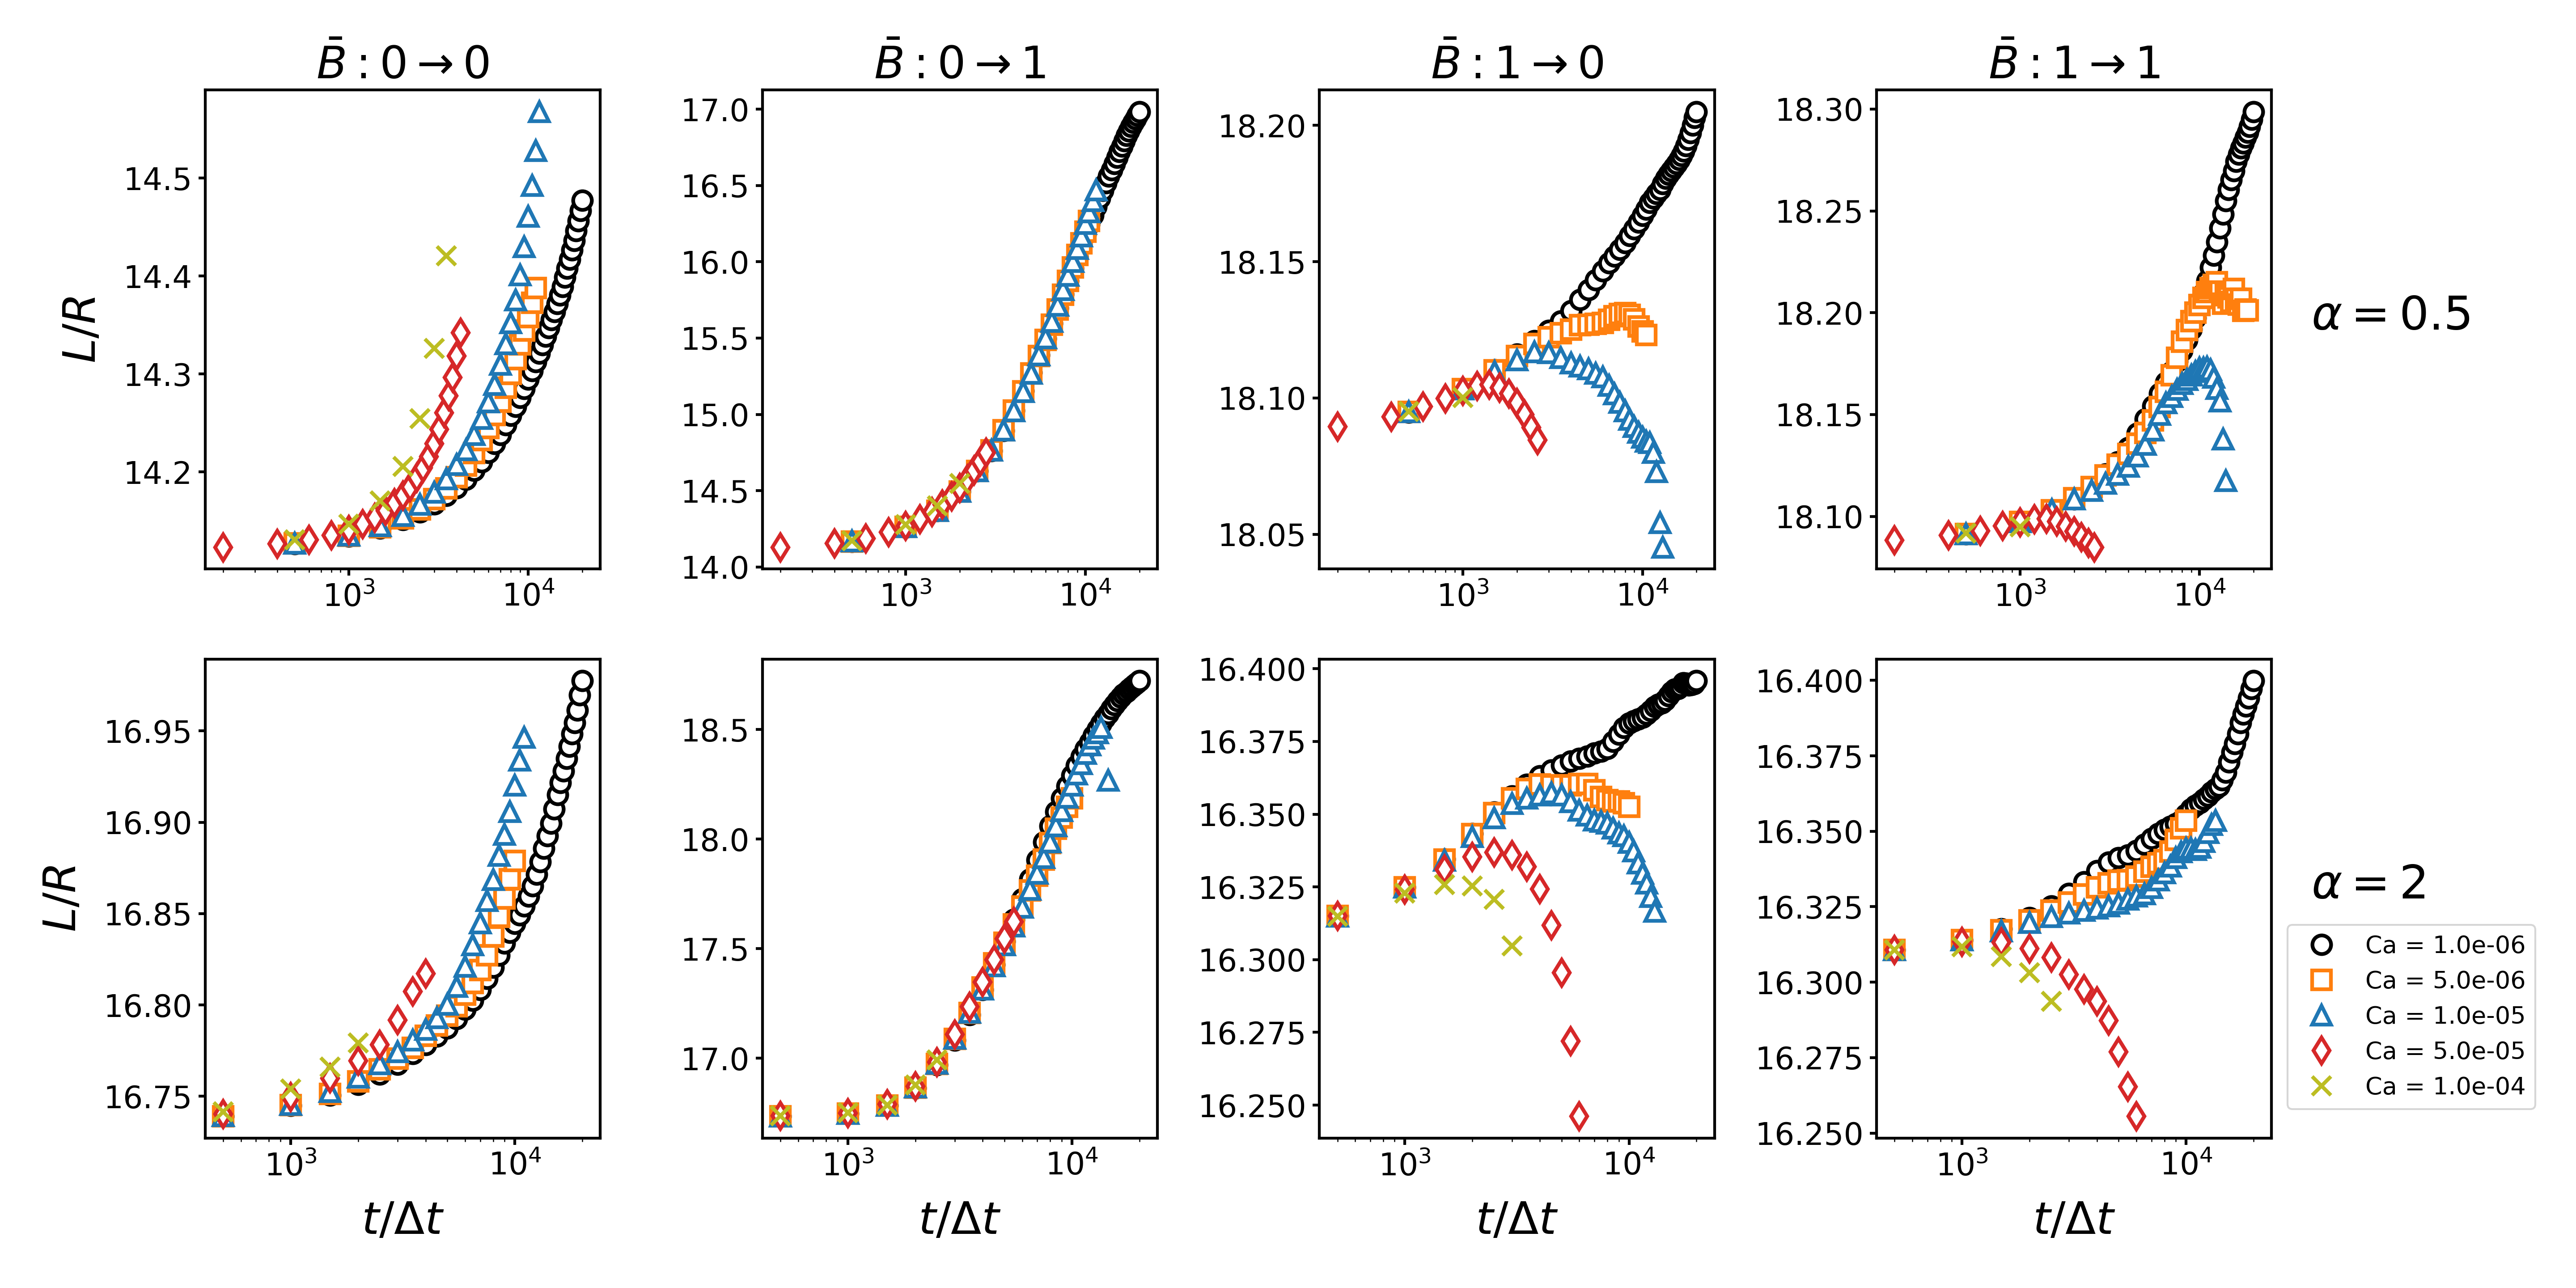
\includegraphics[scale=0.3]{../figures/results/paper3/domain_size-time_compare.png} 
%     \caption{Comparisons of the time evolution of the average domain size for bijels stabilized by ellipsoidal particles undergoing
%              various shear rates under four processes. Initially, the domain size coarsens for all runs under applied shear before
%              reducing in some cases.} 
%     \label{fig:domain_size_time_shear} 
% \end{figure}

% From Figure \ref{fig:domain_size_time_shear}, domains coarsen with time in all cases. When increasing the applied magnetic field in the case of 
% $\bar{B}:0 \rightarrow 1$, I see shear assisted domain coarsening characterized as a 20 \% and 10 \% increase in the domain size of bijels
% stabilized by oblate and prolate particles respectively. This is approximately 5 times greater than the response observed in Figure \ref{fig:domain_size-field_on}
% In the  $\bar{B}: 1 \to 0$ and $\bar{B}: 1 \to 1$ cases, an initial plateau in domain size is observed, followed by a divergence in 
% growth depending on $Ca$. The shear rate appears to influence domain coarsening, with higher $Ca_s$ leading to delayed or 
% suppressed growth, especially in the presence of a field. The difference between applying $\bar{B}: 0 \to 1$ and 
% removing $\bar{B}: 1 \to 0$ the field demonstrates the stability of the particle monolayer when a field is switched off.
% There is little difference in the qualitative trends of domain size change for bijels stabilized with oblate or prolate particles.
% To characterize whether the domain size coarsening observed arises from different phenomena in each case, the area averaged curvature is plotted.